\documentclass[11pt]{article}

\usepackage{fullpage, tikz}
\usetikzlibrary{shapes.geometric, arrows}
\usepackage{wrapfig}
\usepackage{caption}

% Define styles
\tikzstyle{startstop} = [rectangle, rounded corners, minimum width=3cm, minimum height=1cm, text centered, draw=black, fill=red!30]
\tikzstyle{process} = [rectangle, minimum width=2cm, minimum height=1cm, text centered, draw=black, fill=orange!30]
\tikzstyle{nobox} = [minimum width=3cm, minimum height=1cm, text centered, draw=none]
\tikzstyle{arrow} = [thick,->]
\tikzstyle{dottedline} = [thick, dotted]
\captionsetup{justification=centering}

\begin{document}
\title{Group 51 Final Report}
\author{Lewen Oh, Xi Ting Hoh, Yuhan Wu, Jamin Son}
\maketitle
\section{Assembler}
\begin{wrapfigure}{r}{0.5\textwidth}
    \centering
    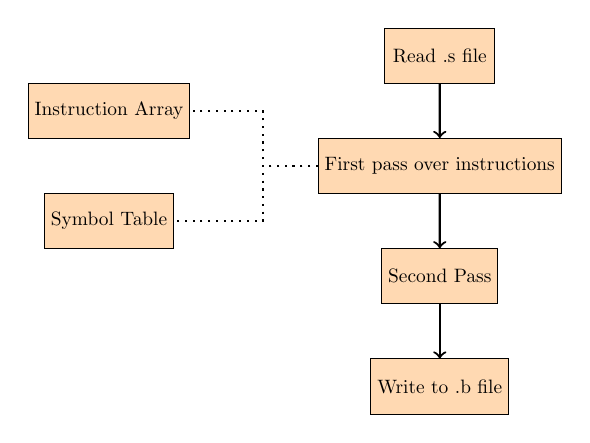
\begin{tikzpicture}[node distance=2cm, scale=0.7, every node/.style={transform shape}]

    \node (reading) [process] {Read .s file};
    \node (first_pass) [process, below of=reading] {First pass over instructions};
    \node (instruction_array) [process, left of=first_pass, yshift=1cm, xshift=-4cm] {Instruction Array};
    \node (second_pass) [process, below of=first_pass] {Second Pass};
    \node (symbol_table) [process, left of=first_pass, yshift = -1cm, xshift=-4cm] {Symbol Table};
    \node (binary_write) [process, below of=second_pass] {Write to .b file};

    \draw [arrow] (reading) -- (first_pass);
    \draw [arrow] (first_pass) -- (second_pass);
    \draw [arrow] (second_pass) -- (binary_write);
    \draw [dottedline] (first_pass.west) -- ++(-1cm,0) |- (instruction_array.east);
    \draw [dottedline] (first_pass.west) -- ++(-1cm,0) |- (symbol_table.east);

    \end{tikzpicture}
    \caption{Flowchart for reading a .s file and processing instructions.}
    \label{fig:process-flowchart}
\end{wrapfigure}

The high-level structure of the assembler is equivalent to the emulator. Both read input files, process and write output. We implemented the assembler using two-passes over the instructions. A broad overview of the assembler is shown to the right. The symbol table and instruction arrays were implemented as classic array data structures with a size and data field.\\
\textbf{First Pass:} During the first pass each line of assembly is: classified to what instruction it is: (and, subs, mul...); and, tokenised to an array of strings. Relevant files: first\_pass.c\\
\textbf{Second Pass:} Each tokenised instruction is encoded to binary. The tokenised array was designed for ease of processing in the second pass. Relevant files: second\_pass.c\\
\\
\textbf{Tokenisation} (fig.2) Load, Store instructions posed extra complexity as there were 4 types: Post-Index, Pre-Index, Unsigned offset and other.\\
\begin{figure}[h]
    \centering
    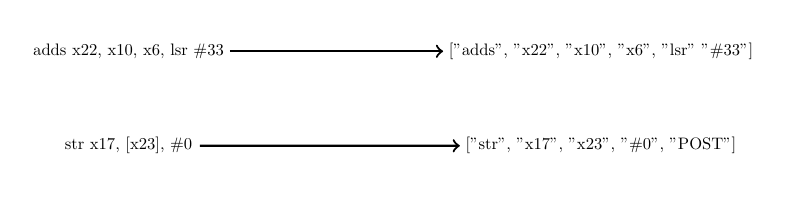
\begin{tikzpicture}[node distance=2cm, scale=0.6, every node/.style={transform shape}, xshift=2cm] % Shift the graph to the right by 2cm

    \node (add) [nobox] {adds	x22, x10, x6, lsr \#33};
    \node (token_add) [nobox, right of=add, xshift=8cm] {["adds", "x22", "x10", "x6", "lsr" "\#33"]};
    \node (str) [nobox, below of=add] {str	x17, [x23], \#0};
    \node (token_str) [nobox, right of=str, xshift=8cm] {["str", "x17", "x23", "\#0", "POST"]};

    \draw[arrow] (add) -- (token_add);
    \draw[arrow] (str) -- (token_str);

    \end{tikzpicture}
    \caption{How assembly instructions are tokenised}
    \label{fig:scp-flowchart}
\end{figure}\\
\textbf{Adding label to symbol table} (fig.3) In first pass, when a label is come across it is added to the symbol table structure with its address calculated using its position within the instructions.
\begin{figure}[t]
    \centering
    \begin{tikzpicture}[node distance=2cm, scale=0.6, every node/.style={transform shape}, xshift=2cm] % Shift the graph to the right by 2cm

    \node (label) [nobox, below of=str] {beef:};
    \node (symbol_entry) [nobox, below of=token_str] {["beef", 0x4]};
    \draw[arrow] (label) -- (symbol_entry);

    \end{tikzpicture}
    \caption{How label instructions were added to the symbol table}
    \label{fig:scp-flowchart}
\end{figure}
\\
\section{Raspberry Pi}
Circuit: We researched how to connect the LED to the Raspberry Pi - the cathode connects to a ground pin via a 220 Ohm resistor, and the anode connects to the desired pin. -> Diagram\\
Debug process: We used our emulator with GDB, putting a breakpoint at the end of each execution loop, so that the contents of registers and memory could be checked. Through this we found 2 issues:\\
\\\textbf{Register size:} We used x registers for all instructions, but this caused a problems loading the correct base address from the .int directives. 0x80003f200000 would be loaded instead of 0x3f200000, as 0x8000 was the .int  directive that came directly after the address .int. Thus, we changed all registers to w registers.\\
\textbf{.int directives:} Initially these were placed at the beginning of the assembly code, meaning the processor would try to execute these first. These were moved to the end of the code.


\section{Extension}
Our extension, inspired by Bandai’s Tamagotchi, is a virtual pet game that is played in the terminal that requires minimal attention. Players can open the game and have the game open in a small terminal beside their work. The pet has happiness and fullness stats that will decrease as time goes on and players will have to interact with it to keep it happy and full. Occasionally, the pet will have to go to the toilet or fall sick, and players will have to clean up after it or feed it medicine.\\\\
\textbf{Design:}
The game is built using a supplementary C library, ncurses, that allows printing to the terminal while the game is running and refreshing the display, among other functions, which would not be possible since our program requires continuously printing to the terminal and taking inputs while the program is running.
Before any programming started, we decided to draw up a flowchard of how the game would function, and we used that as a guide while programming. However, the more we programmed the more we found that additional features were required to complete the game, and thus we needed to keep creating functions as time went on.
Another challenge was making the sprite into a global variable that could be accessed by more than one file/function. We eventually found a solution: one header file, one source file that defines it, and using extern by other source files that need to access it.
In the main function, making the sprite animation on the home screen constantly move while allowing the program to be always open to taking input (using ncurses’ getchar() function) was a difficult issue for us to solve. Ultimately, we took advantage of ncurses’ built in nodelay() function, allows getch() to be skipped if there is no input, and concurrency to display the changing frames of the sprite without interruption, which may cause an error.\\
\textbf{Testing: }
It was difficult for us to test the game as a whole; we focused on testing the behaviour of the individual functions. For example, for the function that prints the sprite, our test was to run the function and see if the result is as we want it to be. For the function that decreases the stats over time, we set the time intervals to seconds instead of minutes, and the original stats to end cases to check that it decreased on time and that it did not decrement past 0.
Admittedly, this method of testing is not as thorough as it should be, though it is effective enough to ensure the basic functionality of the game as the game itself is not very complex.



\section{Reflection}
Group:
We had good communication and split up tasks well based on everyone's strengths. Next time I think we should spend longer talking about the overall big picture of what we need from each other, e.g. parameter data types and return types, so that we wont have to spend as long stitching our tasks together so that everyone's functions/typedefs would come together. This issue stemmed from our initial undersight with Git, and it will definitely be something we implement next time before branching separate ways.\\\\
\textbf{Yuhan:} I think everyone in our group meshed super well, we all balance each other out. This meant we worked great together, with each part we completed being more efficient than the last, but also it made the whole experience fun! I learnt that my weaknesses lie in the aspects of C that require specific knowledge of functions/libraries. For example, I struggle with reading from and writing to files and strings, whereas I’m stronger in the more logical aspects, where knowledge of libraries and functions isn’t necessary. \\
\textbf{Xi Ting:} I felt that I could express myself very genuinely and confidently in this team and knowing my voice was heard made me more confident to vocalise my ideas as well as my agreements and disagreements.  At first, I was worried that I would not be as productive as the other members as programming is not my strength, though I felt that I made up for it with my positivity and by generating creative ideas, especially for the extension. Through this project, I learned the valuable lesson of playing to my strengths to complement my weakness, something I will be applying to all of my future group projects.\\
\textbf{Lewen:} Most of my programming experience lies with solving logic-based problems, however this project introduced the need to deal with file I/O and building C projects, which I had no prior experience of. I was delegated these two tasks, and although I initially was intimidated with these unexplored technical areas, in hindsight I am grateful for having done this, as I had to learn a lot from scratch. Although I still believe my strengths lie in the logical side of programming, this experience definitely gave me more courage to go out of my comfort zone to learn more technical programming skills. In future group projects, I believe that this would be a key practice to maintain consistent and efficient progress.\\
\textbf{Jamin:} This project was incredibly enjoyable and informative. Due to my position as leader, I knew that I largely responsible for the timely execution and quality of the project. Team discussions were frequently used to coordinate tasks and interconnected components; and also to make sure everyone knew the fundamentals correctly. I enjoyed thinking about the technical skill sets and personality qualities of each team members and find the right fit between members. I found out that as leader, I was not able to just focus on my coding task, but had to consistently spend time figuring out the steps ahead so that I was always prepared to delegate tasks.
An aspect I would change is the philosophy to build quicker and test more often. Sometimes I caught myself attempting to make things perfect the first time causing delays in production.
\end{document}
